\documentclass[12pt, xcolor=dvipsnames,svgnames,x11names]{article}
\usepackage{xcolor}
\usepackage{amsmath}
%\usepackage{universityos}
\usepackage{xspace}
\usepackage{url}
\usepackage[colorlinks=true,bookmarks=false,linkcolor=black,urlcolor=blue,citecolor=black]{hyperref}
\usepackage{minted}
\usepackage{fancyhdr}
\usepackage[top=1in,bottom=1in,left=1in,right=1in]{geometry}
\usepackage{multicol}
\usepackage{pgfplots}
\usetikzlibrary{circuits.logic.US}
% \usepackage{tgschola}
\let\temp\rmdefault
\usepackage{mathpazo}
\let\rmdefault\temp

\definecolor{roseRed}{HTML}{e20047}
\definecolor{coolGray}{HTML}{474747} % Neutral gray to contrast roseRed
\definecolor{mocha}{HTML}{a47864}
\definecolor{sage}{HTML}{8a9a5b}
\definecolor{dustyblue}{HTML}{6e8ca0}
\definecolor{terracotta}{HTML}{c87f5b}
\definecolor{lavender}{HTML}{9d8bb0}
\definecolor{darkmocha}{HTML}{7a5a4b}
\definecolor{darksage}{HTML}{667244}
\definecolor{darkdustyblue}{HTML}{526878}
\definecolor{darkterracotta}{HTML}{9e6347}
\definecolor{darklavender}{HTML}{766688}
\definecolor{winery}{HTML}{7e212a}

\definecolor{lightmocha}{HTML}{c2a190}
\definecolor{lightmocha1}{HTML}{d1b09c}
\definecolor{lightmocha2}{HTML}{e2c4b0}
\definecolor{lightmocha3}{HTML}{f0d9c7}

\definecolor{androidBlue}{HTML}{8AB4F8}
\definecolor{androidBlueLight}{HTML}{E8F0FE}
\definecolor{androidGreen}{HTML}{81C995}
\definecolor{androidGreenLight}{HTML}{E6F4EA}

% Red variants - based on Android's "error" and warning colors
\definecolor{androidRed}{HTML}{F28B82}
\definecolor{androidRedLight}{HTML}{FADAD7}

% Yellow variants - based on Android's accent/warning colors
\definecolor{androidYellow}{HTML}{FDD663}
\definecolor{androidYellowLight}{HTML}{FEF7E0}

% Purple variants - based on Android's system UI accents
\definecolor{androidPurple}{HTML}{D7AEFB}
\definecolor{androidPurpleLight}{HTML}{F4EAFC}

% Orange variants - based on Android's notification colors
\definecolor{androidOrange}{HTML}{FCAD70}
\definecolor{androidOrangeLight}{HTML}{FEEADC}

% Teal variants - based on Android's Material You palette
\definecolor{androidTeal}{HTML}{78D9EC}
\definecolor{androidTealLight}{HTML}{E6F6F9}

% Gray variants - based on Android's neutral colors
\definecolor{androidGray}{HTML}{DADCE0}
\definecolor{androidGrayLight}{HTML}{F1F3F4}

\usepackage{biolinum} % included with the {Libertine} font package
\renewcommand{\familydefault}{\sfdefault}

\definecolor{plum}{cmyk}{0.50,1,0,0}

\usepackage[many]{tcolorbox}
\usepackage{CJKutf8}

\newcommand{\hw}{Classwork 07: Building Blocks for Continuous-Time Signals}
\newcommand{\duedate}{September 16, 2026}


% Redefine \maketitle to include tcolorbox
\makeatletter
\renewcommand{\maketitle}{%
    \begin{center}
        \begin{tcolorbox}[
            enhanced,
            colback=white,
            colframe=red!70!black,
            arc=0mm,
            title={\textcolor{white}{\bfseries CPE 381 \@title}},
            coltitle=white,
            fonttitle=\bfseries\large,
            attach boxed title to top left={xshift=10pt, yshift=-\tcboxedtitleheight/2},
            boxed title style={
            sharp corners,
            colback=red!70!black,
            frame hidden,
            boxrule=0pt,
            left=10pt, right=10pt,
            top=3pt, bottom=3pt
            }
        ]
        \large
        \vspace{10pt}
        \noindent Student Name (as in Canvas): \underline{\hspace{8cm}} 
        
        \vspace{10pt}
        \noindent A Number: \underline{\hspace{12cm}}

        \vspace{10pt}
        \noindent Points: 20 \quad Duration: 15 minutes \hfill \quad Due:~\duedate  ~(In-Class)

            \end{tcolorbox}
    \end{center}
}
\makeatother

\setlength{\parindent}{0pt}
\setlength{\parskip}{4pt}%

\usepackage{tikz}
\usepackage{pgfplots}

\newcommand{\coursenumber}{CPE381}
\newcommand{\courseyear}{2026\xspace}
\newcommand{\coursedatetime}{Mon/Wed 11:20 AM -- 12:40 PM\xspace}
\newcommand{\coursetitle}{Signals and Systems for Computer Engineers\xspace}
\newcommand{\courseterm}{Fall, \courseyear}
\newcommand{\courseurl}{\url{http://uah.instructure.com/}}
\newcommand{\courselocation}{ENG 207\xspace}
\newcommand{\courselocationurl}{TBD}

\newcommand{\instructorname}{Rahul Bhadani\xspace}
\newcommand{\instructoremail}{\href{mailto:rahul.bhadani@uah.edu}{rahul.bhadani@uah.edu}}
\newcommand{\instructoroffice}{ENG 217-H\xspace}
\newcommand{\instructorofficehours}{Mon/Tue/Wed 2:00 PM - 4:00 PM}


% \everymath{\color{Navy}}
\everydisplay{\color{roseRed}}
\usepackage{sectsty}
\sectionfont{\color{dustyblue}}  % sets colour of sections
\subsectionfont{\color{terracotta}}  % sets colour of sections
\subsubsectionfont{\color{lavender}}  % sets colour of sections


\def\m@th{\normalcolor\mathsurround\z@}

\setlength{\parskip}{\baselineskip}%
\setlength{\parindent}{0pt}%

%%%%%%%%%%%%%%%%%%%%%%%%%%%%%%%%%%%%%%%%%%%%%%%%%%%%%%%%%%%%%%%%%%%%%


\def\e{{\textrm{e}}}
\def\d{\textrm{d}}
\def\T{{\textsf{T}}}
\def\sech{{\textrm{sech}}}
\def\x{{\mathbf x}}

\def\++{{$^{++}$}}

\def\Abb{{\mathbb A}}
\def\Bbb{{\mathbb B}}
\def\Cbb{{\mathbb C}}
\def\Dbb{{\mathbb D}}
\def\Ebb{{\mathbb E}}
\def\Fbb{{\mathbb F}}
\def\Gbb{{\mathbb G}}
\def\Hbb{{\mathbb H}}
\def\Ibb{{\mathbb I}}
\def\Jbb{{\mathbb J}}
\def\Kbb{{\mathbb K}}
\def\Lbb{{\mathbb L}}
\def\Mbb{{\mathbb M}}
\def\Nbb{{\mathbb N}}
\def\Obb{{\mathbb O}}
\def\Pbb{{\mathbb P}}
\def\Qbb{{\mathbb Q}}
\def\Rbb{{\mathbb R}}
\def\Sbb{{\mathbb S}}
\def\Tbb{{\mathbb T}}
\def\Ubb{{\mathbb U}}
\def\Vbb{{\mathbb V}}
\def\Wbb{{\mathbb W}}
\def\Xbb{{\mathbb X}}
\def\Ybb{{\mathbb Y}}
\def\Zbb{{\mathbb Z}}



\def\Acal{{\mathcal A}}
\def\Bcal{{\mathcal B}}
\def\Ccal{{\mathcal C}}
\def\Dcal{{\mathcal D}}
\def\Ecal{{\mathcal E}}
\def\Fcal{{\mathcal F}}
\def\Gcal{{\mathcal G}}
\def\Hcal{{\mathcal H}}
\def\Ical{{\mathcal I}}
\def\Jcal{{\mathcal J}}
\def\Kcal{{\mathcal K}}
\def\Lcal{{\mathcal L}}
\def\Mcal{{\mathcal M}}
\def\Ncal{{\mathcal N}}
\def\Ocal{{\mathcal O}}
\def\Pcal{{\mathcal P}}
\def\Qcal{{\mathcal Q}}
\def\Rcal{{\mathcal R}}
\def\Scal{{\mathcal S}}
\def\Tcal{{\mathcal T}}
\def\Ucal{{\mathcal U}}
\def\Vcal{{\mathcal V}}
\def\Wcal{{\mathcal W}}
\def\Xcal{{\mathcal X}}
\def\Ycal{{\mathcal Y}}
\def\Zcal{{\mathcal Z}}

\def\abf{{\mathbf a}}
\def\bbf{{\mathbf b}}
\def\cbf{{\mathbf c}}
\def\dbf{{\mathbf d}}
\def\ebf{{\mathbf e}}
\def\fbf{{\mathbf f}}
\def\gbf{{\mathbf g}}
\def\hbf{{\mathbf h}}
\def\ibf{{\mathbf i}}
\def\jbf{{\mathbf j}}
\def\kbf{{\mathbf k}}
\def\lbf{{\mathbf l}}
\def\mbf{{\mathbf m}}
\def\nbf{{\mathbf n}}
\def\obf{{\mathbf o}}
\def\pbf{{\mathbf p}}
\def\qbf{{\mathbf q}}
\def\rbf{{\mathbf r}}
\def\sbf{{\mathbf s}}
\def\tbf{{\mathbf t}}
\def\ubf{{\mathbf u}}
\def\vbf{{\mathbf v}}
\def\wbf{{\mathbf w}}
\def\xbf{{\mathbf x}}
\def\ybf{{\mathbf y}}
\def\zbf{{\mathbf z}}

\def\Abf{{\mathbf A}}
\def\Bbf{{\mathbf B}}
\def\Cbf{{\mathbf C}}
\def\Dbf{{\mathbf D}}
\def\Ebf{{\mathbf E}}
\def\Fbf{{\mathbf F}}
\def\Gbf{{\mathbf G}}
\def\Hbf{{\mathbf H}}
\def\Ibf{{\mathbf I}}
\def\Jbf{{\mathbf J}}
\def\Kbf{{\mathbf K}}
\def\Lbf{{\mathbf L}}
\def\Mbf{{\mathbf M}}
\def\Nbf{{\mathbf N}}
\def\Obf{{\mathbf O}}
\def\Pbf{{\mathbf P}}
\def\Qbf{{\mathbf Q}}
\def\Rbf{{\mathbf R}}
\def\Sbf{{\mathbf S}}
\def\Tbf{{\mathbf T}}
\def\Ubf{{\mathbf U}}
\def\Vbf{{\mathbf V}}
\def\Wbf{{\mathbf W}}
\def\Xbf{{\mathbf X}}
\def\Ybf{{\mathbf Y}}
\def\Zbf{{\mathbf Z}}

\def\phat{{\hat p}}

\usepackage{amsmath}
\DeclareMathOperator*{\argmax}{arg\,max}
\DeclareMathOperator*{\argmin}{arg\,min}

\def\xbar{{\overline x}}
\def\ybar{{\overline y}}
\def\e{{\textrm{e}}}
\def\d{\textrm{d}}
\def\T{{\textsf{T}}}
\def\sech{{\textrm{sech}}}
\def\x{{\mathbf x}}

\def\++{{$^{++}$}}

\def\Abb{{\mathbb A}}
\def\Bbb{{\mathbb B}}
\def\Cbb{{\mathbb C}}
\def\Dbb{{\mathbb D}}
\def\Ebb{{\mathbb E}}
\def\Fbb{{\mathbb F}}
\def\Gbb{{\mathbb G}}
\def\Hbb{{\mathbb H}}
\def\Ibb{{\mathbb I}}
\def\Jbb{{\mathbb J}}
\def\Kbb{{\mathbb K}}
\def\Lbb{{\mathbb L}}
\def\Mbb{{\mathbb M}}
\def\Nbb{{\mathbb N}}
\def\Obb{{\mathbb O}}
\def\Pbb{{\mathbb P}}
\def\Qbb{{\mathbb Q}}
\def\Rbb{{\mathbb R}}
\def\Sbb{{\mathbb S}}
\def\Tbb{{\mathbb T}}
\def\Ubb{{\mathbb U}}
\def\Vbb{{\mathbb V}}
\def\Wbb{{\mathbb W}}
\def\Xbb{{\mathbb X}}
\def\Ybb{{\mathbb Y}}
\def\Zbb{{\mathbb Z}}



\def\Acal{{\mathcal A}}
\def\Bcal{{\mathcal B}}
\def\Ccal{{\mathcal C}}
\def\Dcal{{\mathcal D}}
\def\Ecal{{\mathcal E}}
\def\Fcal{{\mathcal F}}
\def\Gcal{{\mathcal G}}
\def\Hcal{{\mathcal H}}
\def\Ical{{\mathcal I}}
\def\Jcal{{\mathcal J}}
\def\Kcal{{\mathcal K}}
\def\Lcal{{\mathcal L}}
\def\Mcal{{\mathcal M}}
\def\Ncal{{\mathcal N}}
\def\Ocal{{\mathcal O}}
\def\Pcal{{\mathcal P}}
\def\Qcal{{\mathcal Q}}
\def\Rcal{{\mathcal R}}
\def\Scal{{\mathcal S}}
\def\Tcal{{\mathcal T}}
\def\Ucal{{\mathcal U}}
\def\Vcal{{\mathcal V}}
\def\Wcal{{\mathcal W}}
\def\Xcal{{\mathcal X}}
\def\Ycal{{\mathcal Y}}
\def\Zcal{{\mathcal Z}}

\def\abf{{\mathbf a}}
\def\bbf{{\mathbf b}}
\def\cbf{{\mathbf c}}
\def\dbf{{\mathbf d}}
\def\ebf{{\mathbf e}}
\def\fbf{{\mathbf f}}
\def\gbf{{\mathbf g}}
\def\hbf{{\mathbf h}}
\def\ibf{{\mathbf i}}
\def\jbf{{\mathbf j}}
\def\kbf{{\mathbf k}}
\def\lbf{{\mathbf l}}
\def\mbf{{\mathbf m}}
\def\nbf{{\mathbf n}}
\def\obf{{\mathbf o}}
\def\pbf{{\mathbf p}}
\def\qbf{{\mathbf q}}
\def\rbf{{\mathbf r}}
\def\sbf{{\mathbf s}}
\def\tbf{{\mathbf t}}
\def\ubf{{\mathbf u}}
\def\vbf{{\mathbf v}}
\def\wbf{{\mathbf w}}
\def\xbf{{\mathbf x}}
\def\ybf{{\mathbf y}}
\def\zbf{{\mathbf z}}

\def\Abf{{\mathbf A}}
\def\Bbf{{\mathbf B}}
\def\Cbf{{\mathbf C}}
\def\Dbf{{\mathbf D}}
\def\Ebf{{\mathbf E}}
\def\Fbf{{\mathbf F}}
\def\Gbf{{\mathbf G}}
\def\Hbf{{\mathbf H}}
\def\Ibf{{\mathbf I}}
\def\Jbf{{\mathbf J}}
\def\Kbf{{\mathbf K}}
\def\Lbf{{\mathbf L}}
\def\Mbf{{\mathbf M}}
\def\Nbf{{\mathbf N}}
\def\Obf{{\mathbf O}}
\def\Pbf{{\mathbf P}}
\def\Qbf{{\mathbf Q}}
\def\Rbf{{\mathbf R}}
\def\Sbf{{\mathbf S}}
\def\Tbf{{\mathbf T}}
\def\Ubf{{\mathbf U}}
\def\Vbf{{\mathbf V}}
\def\Wbf{{\mathbf W}}
\def\Xbf{{\mathbf X}}
\def\Ybf{{\mathbf Y}}
\def\Zbf{{\mathbf Z}}

\def\phat{{\hat p}}
\def\what{{\hat w}}
\def\yhat{{\hat y}}


\newcommand{\answer}{
    \fcolorbox{orange}{PapayaWhip}{
\begin{minipage}{\textwidth}
        \textbf{Answer}
    \end{minipage}
}
}

\newcommand{\codeoutput}[1]{
Output:\\\vspace{5px}
    \fcolorbox{orange}{WhiteSmoke}{
\begin{minipage}{\textwidth}
        { \color{DodgerBlue} 
        
        
       \texttt{#1}
       }
    \end{minipage}
}
}


\newcommand{\orangebox}[1]{
    \fcolorbox{orange}{white}{
\begin{minipage}{\textwidth}
       {\color{MidnightBlue} 
       #1
       }
    \end{minipage}
}
}





% Add showanswer toggle (set to "yes" for solutions, anything else for student version)
\usepackage{ifthen}
\newcommand{\showanswer}{yes}

\pagestyle{fancy}

\lhead{\footnotesize{\coursenumber, \courseterm}, \footnotesize{The University of Alabama in Huntsville}}
\chead{}
\rhead{\footnotesize{\emph{\hw}}}
\lfoot{\footnotesize{Instructor: \instructorname}}
\cfoot{\footnotesize{\thepage}}
\rfoot{\footnotesize{\textit{Last Revised:~\today}}}
\renewcommand{\headrulewidth}{0.1pt}
\renewcommand{\footrulewidth}{0.1pt}
\newcommand{\minipagewidth}{0.8\columnwidth}

\renewcommand{\thefootnote}{\fnsymbol{footnote}}


\renewcommand{\headrulewidth}{0.1pt}
\renewcommand{\footrulewidth}{0.1pt}

\renewcommand{\thefootnote}{\fnsymbol{footnote}}

\usepackage{mdframed} 
\usepackage[american]{circuitikz}

\begin{document}


\title{\textsc{\hw}}

\author{Instructor: \instructorname}
\date{Due: \duedate}

\maketitle

\begin{enumerate}
\item Assuming $u(t)$ is the unit-step function as discussed in the class, sketch $u(t+1)$.


\begin{tcolorbox}[
    enhanced,breakable,
    colback=androidBlueLight!80,
    colframe=androidBlue,
    arc=5pt,
    boxrule=1pt,
    title=\textbf{Answer},
    fonttitle=\bfseries,
    coltitle=black,
    top=10pt,
    bottom=8pt,
    left=8pt,
    right=8pt,
    attach boxed title to top left={xshift=10pt, yshift=-\tcboxedtitleheight/2},
    boxed title style={
    colback=androidBlue,    
        colframe=androidBlue,
        arc=3pt,
        boxrule=0pt,
        left=6pt, right=6pt,
        top=3pt, bottom=3pt
    }
    ]
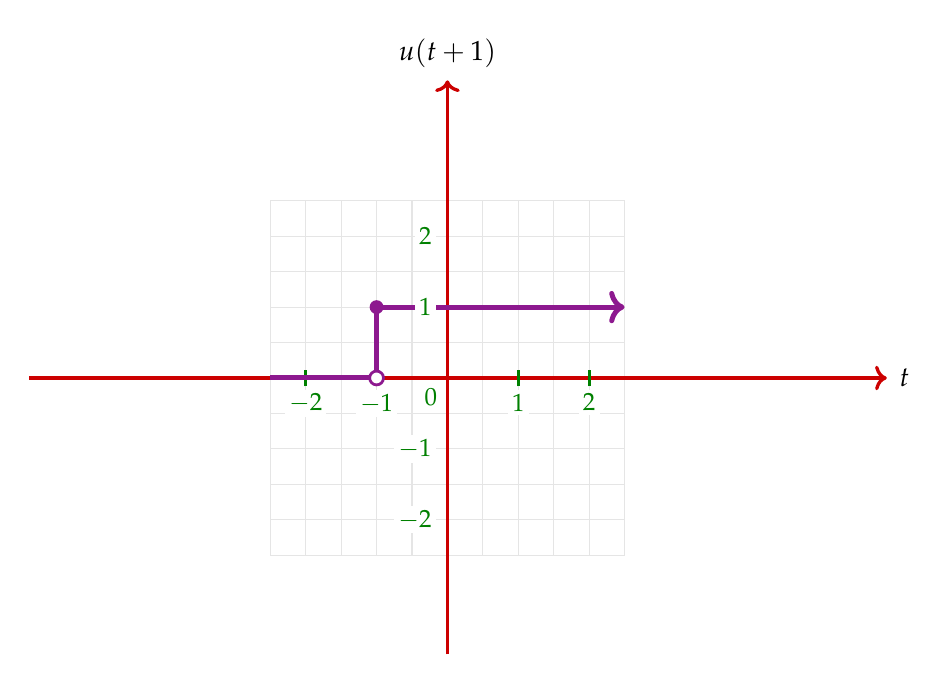
\begin{tikzpicture}[
    x=0.9cm, y=0.9cm,
    axisline/.style={red!80!black, line width=1.2pt, ->},
    lbl/.style={green!50!black, font=\small\bfseries,
                fill=white, inner sep=1.5pt},
    tick/.style={green!50!black, line width=1pt}
]

% ---------- grid, minor cells of half a unit ----------
\draw[lightgray!40, thin, step=0.5] (-2.5,-2.5) grid (2.5,2.5);

% ---------- axes ----------
\draw[axisline] (-5.9,0) -- (6.2,0) node[right, black, inner sep=4pt] {$t$};
\draw[axisline] (0,-3.9) -- (0,4.2) node[above, black, inner sep=4pt] {$u(t+1)$};

% ---------- ticks in all quadrants ----------
\foreach \u in {-2,-1,1,2}
  \draw[tick] ([yshift=-3pt]\u,0) -- ([yshift=3pt]\u,0);
\foreach \v in {-3,-2,-1,1,2,3}
  \foreach \v in {-2,-1,2}
  \node[lbl, left=4pt] at (0,\v) {$\v$};
  
  % ---------- u(t+1): zero for t < -1, one for t >= -1 ----------
\draw[plum, line width=1.8pt] (-2.5,0) -- (-1,0);
\draw[plum, line width=1.8pt] (-1,0) -- (-1,1);
\draw[plum, line width=1.8pt, ->] (-1,1) -- (2.5,1);
\draw[plum, fill=white, line width=1pt] (-1,0) circle (2.5pt);
\fill[plum] (-1,1) circle (2.5pt);

% ---------- tick labels ----------
\foreach \u in {-2,-1,1,2}
  \node[lbl, below=4pt] at (\u,0) {$\u$};
\foreach \v in {-2,-1,1,2}
  \node[lbl, left=4pt] at (0,\v) {$\v$};
\node[lbl, anchor=north east, xshift=-2pt, yshift=-2pt] at (0,0) {$0$};

\end{tikzpicture}

    
\end{tcolorbox}



\item Sketch $x(t) = \sin(t)u(t)$.



\begin{tcolorbox}[
    enhanced,breakable,
    colback=androidBlueLight!80,
    colframe=androidBlue,
    arc=5pt,
    boxrule=1pt,
    title=\textbf{Answer},
    fonttitle=\bfseries,
    coltitle=black,
    top=10pt,
    bottom=8pt,
    left=8pt,
    right=8pt,
    attach boxed title to top left={xshift=10pt, yshift=-\tcboxedtitleheight/2},
    boxed title style={
    colback=androidBlue,    
        colframe=androidBlue,
        arc=3pt,
        boxrule=0pt,
        left=6pt, right=6pt,
        top=3pt, bottom=3pt
    }
    ]

\resizebox{!}{0.35\linewidth}{
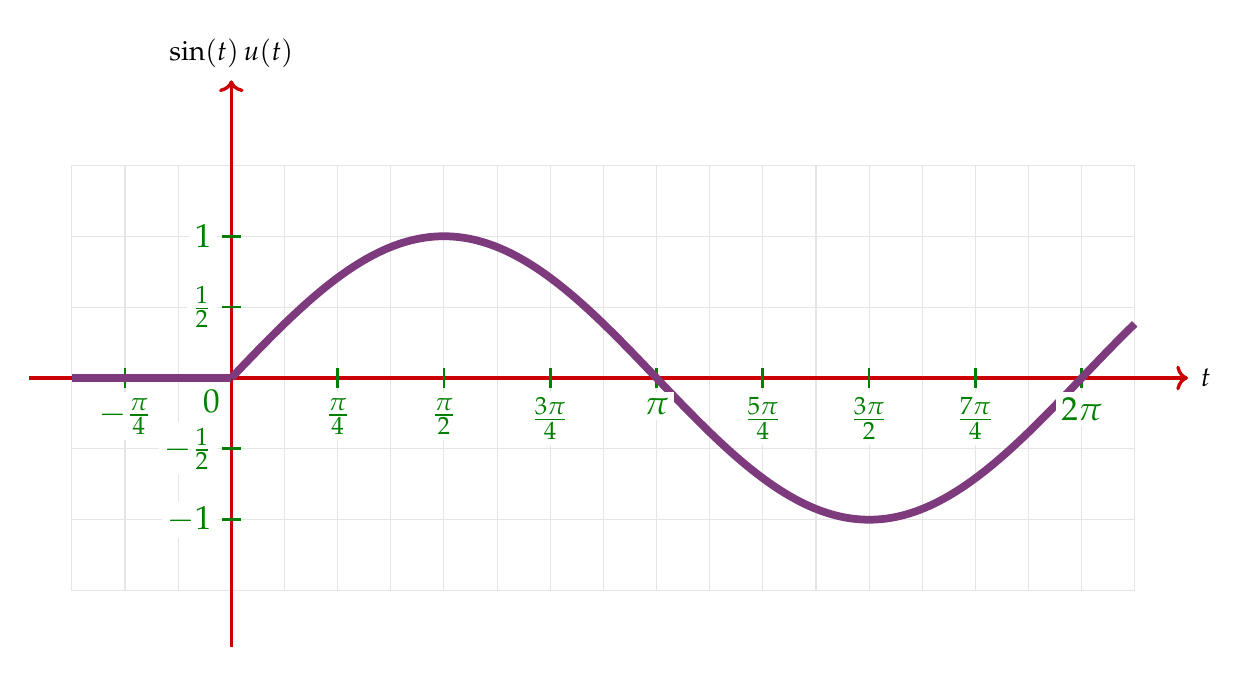
\begin{tikzpicture}[
    x=1.35cm, y=1.8cm,
    axisline/.style={red!80!black, line width=1.2pt, ->},
    lbl/.style={green!50!black, font=\large\bfseries,
                fill=white, inner sep=2pt},
    tick/.style={green!50!black, line width=1pt}
]

% One horizontal unit is pi/4.  One vertical unit is 1.
\draw[lightgray!40, thin, step=0.5] (-1.5,-1.5) grid (8.5,1.5);

\draw[axisline] (-1.9,0) -- (9.0,0) node[right, black, inner sep=4pt] {$t$};
\draw[axisline] (0,-1.9) -- (0,2.1) node[above, black, inner sep=4pt]
      {$\sin(t)\,u(t)$};

% ---------- ticks ----------
\foreach \u in {-1,1,2,3,4,5,6,7,8}
  \draw[tick] ([yshift=-3.5pt]\u,0) -- ([yshift=3.5pt]\u,0);
\foreach \v in {-1,-0.5,0.5,1}
  \draw[tick] ([xshift=-3.5pt]0,\v) -- ([xshift=3.5pt]0,\v);

% ---------- x(t) = sin(t) u(t) ----------
\draw[plum!70!black, line width=2.8pt] (-1.5,0) -- (0,0);
\draw[plum!70!black, line width=2.8pt, smooth]
      plot[domain=0:8.5, samples=150] (\x, {sin(\x*45)});
      
% ---------- tick labels, multiples of pi/4 ----------
\foreach \u/\txt in {%
    -1/{-\tfrac{\pi}{4}}, 1/{\tfrac{\pi}{4}}, 2/{\tfrac{\pi}{2}},
     3/{\tfrac{3\pi}{4}}, 4/{\pi}, 5/{\tfrac{5\pi}{4}},
     6/{\tfrac{3\pi}{2}}, 7/{\tfrac{7\pi}{4}}, 8/{2\pi}}
  \node[lbl, below=5pt] at (\u,0) {$\txt$};

\node[lbl, left=5pt] at (0,1)    {$1$};
\node[lbl, left=5pt] at (0,0.5)  {$\tfrac{1}{2}$};
\node[lbl, left=5pt] at (0,-0.5) {$-\tfrac{1}{2}$};
\node[lbl, left=5pt] at (0,-1)   {$-1$};
\node[lbl, anchor=north east, xshift=-2pt, yshift=-2pt] at (0,0) {$0$};

\end{tikzpicture}
}    
\end{tcolorbox}

\item Write mathematical equation corresponding to the following graph.

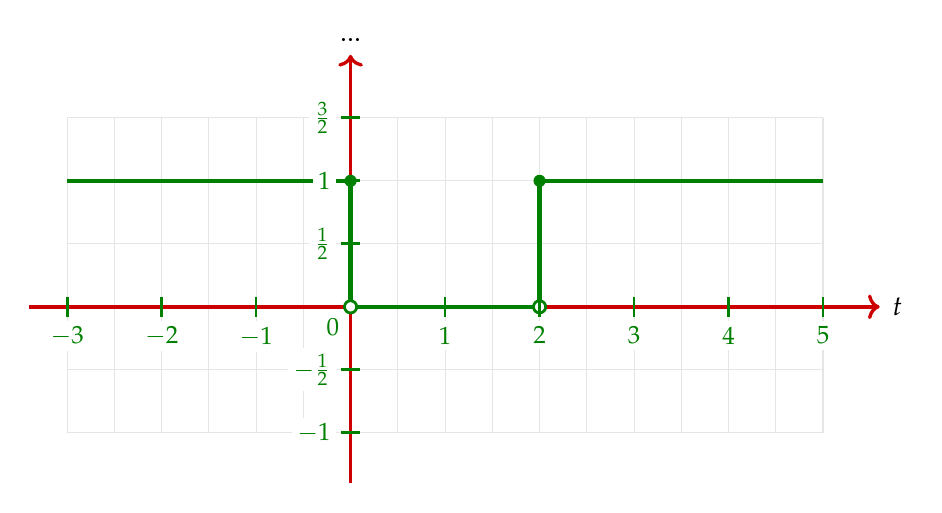
\begin{tikzpicture}[
    x=1.2cm, y=1.6cm,
    axisline/.style={red!80!black, line width=1.2pt, ->},
    curve/.style={green!50!black, line width=1.6pt},
    lbl/.style={green!50!black, font=\small\bfseries,
                fill=white, inner sep=2pt},
    tick/.style={green!50!black, line width=1pt}
]

% ---------- grid ----------
\draw[lightgray!40, thin, step=0.5] (-3,-1) grid (5,1.5);

% ---------- axes ----------
\draw[axisline] (-3.4,0) -- (5.6,0) node[right, black, inner sep=4pt] {$t$};
\draw[axisline] (0,-1.4) -- (0,2.0) node[above, black, inner sep=4pt]
      {$...$};

% ---------- signal ----------
\draw[curve] (-3,1) -- (0,1) -- (0,0) -- (2,0) -- (2,1) -- (5,1);

% ---------- jump endpoints, u(0)=1 ----------
\foreach \p in {(0,1),(2,1)}
  \fill[green!50!black] \p circle (2.2pt);
\foreach \p in {(0,0),(2,0)}
  \draw[green!50!black, line width=1pt, fill=white] \p circle (2.2pt);

% ---------- ticks ----------
\foreach \u in {-3,-2,-1,1,2,3,4,5}
  \draw[tick] ([yshift=-3.5pt]\u,0) -- ([yshift=3.5pt]\u,0);
\foreach \v in {-1,-0.5,0.5,1,1.5}
  \draw[tick] ([xshift=-3.5pt]0,\v) -- ([xshift=3.5pt]0,\v);

% ---------- tick labels ----------
\foreach \u in {-3,-2,-1,1,2,3,4,5}
  \node[lbl, below=5pt] at (\u,0) {$\u$};
\node[lbl, left=5pt] at (0,1.5)  {$\tfrac{3}{2}$};
\node[lbl, left=5pt] at (0,1)    {$1$};
\node[lbl, left=5pt] at (0,0.5)  {$\tfrac{1}{2}$};
\node[lbl, left=5pt] at (0,-0.5) {$-\tfrac{1}{2}$};
\node[lbl, left=5pt] at (0,-1)   {$-1$};
\node[lbl, anchor=north east, xshift=-2pt, yshift=-2pt] at (0,0) {$0$};

\end{tikzpicture}

\begin{tcolorbox}[
    enhanced,breakable,
    colback=androidBlueLight!80,
    colframe=androidBlue,
    arc=5pt,
    boxrule=1pt,
    title=\textbf{Answer},
    fonttitle=\bfseries,
    coltitle=black,
    top=10pt,
    bottom=8pt,
    left=8pt,
    right=8pt,
    attach boxed title to top left={xshift=10pt, yshift=-\tcboxedtitleheight/2},
    boxed title style={
    colback=androidBlue,    
        colframe=androidBlue,
        arc=3pt,
        boxrule=0pt,
        left=6pt, right=6pt,
        top=3pt, bottom=3pt
    }
    ]

$u(t-2)+u(-t)$
    
\end{tcolorbox}


\item Calculate the energy of the signal 

\begin{align*}
z(t) & = \begin{cases}
1, \quad 0 \leq t \leq 10\\
0, \quad \text{otherwise}
\end{cases}
\end{align*}

\begin{tcolorbox}[
    enhanced,breakable,
    colback=androidBlueLight!80,
    colframe=androidBlue,
    arc=5pt,
    boxrule=1pt,
    title=\textbf{Answer},
    fonttitle=\bfseries,
    coltitle=black,
    top=10pt,
    bottom=8pt,
    left=8pt,
    right=8pt,
    attach boxed title to top left={xshift=10pt, yshift=-\tcboxedtitleheight/2},
    boxed title style={
    colback=androidBlue,    
        colframe=androidBlue,
        arc=3pt,
        boxrule=0pt,
        left=6pt, right=6pt,
        top=3pt, bottom=3pt
    }
    ]


Energy of the signal is given by

\begin{align*}
E_z & = \int_{-\infty}^\infty |z(t)|^2 dt = \int_0^{10} |1|^2 dt =  \int_0^{10} 1 dt = [t]_{t=0}^{t=10} = 10-0 = 10
\end{align*}

Note that integral bounds changes from $\pm \infty $ to $[0, 10]$ due to signa's definition provided in the qestion. The signal is zero outside $t = [0, 10]$.

\end{tcolorbox}



\end{enumerate}

\end{document}